\documentclass[11pt]{article} % For LaTeX2e
\usepackage{rldmsubmit,palatino}
\usepackage{graphicx}

\title{Inverse Modular Reinforcement Learning on Human Motion}

\author{
Shun Zhang\\
Department of Computer Science\\
University of Texas at Austin\\
Austin, TX 78712 \\
\texttt{menie482@cs.utexas.edu} \\
\And
Matthew Tong \\
Center for Perceptual Systems\\
University of Texas at Austin\\
Austin, TX 78712 \\
\texttt{mhtong@gmail.com} \\
\AND
Mary Hayhoe \\
Center for Perceptual Systems\\
University of Texas at Austin\\
Austin, TX 78712 \\
\texttt{hayhoe@utexas.edu} \\
\And
Dana Ballard \\
Department of Computer Science\\
University of Texas at Austin\\
Austin, TX 78712 \\
\texttt{dana@cs.utexas.edu} \\
\\
}

% The \author macro works with any number of authors. There are two commands
% used to separate the names and addresses of multiple authors: \And and \AND.
%
% Using \And between authors leaves it to \LaTeX{} to determine where to break
% the lines. Using \AND forces a linebreak at that point. So, if \LaTeX{}
% puts 3 of 4 authors names on the first line, and the last on the second
% line, try using \AND instead of \And before the third author name.

\newcommand{\fix}{\marginpar{FIX}}
\newcommand{\new}{\marginpar{NEW}}

\begin{document}

\maketitle

\begin{abstract}
%The \emph{abstract} should be a maximum of 2000 characters of text, including
%spaces (no figure is allowed).
\end{abstract}

\keywords{
enter key words here
}

\acknowledgements{}

\startmain % to start the main 1-4 pages of the submission.

\section{Introduction}

Human is able to learn complicated behaviors much faster than machines can do.

We analyze human's behavior of accomplishing various tasks. With the best of our
knowledge, there is no work using inverse reinforcement learning to understand
human motional behavior in the literature.

We conduct this research motivated by two questions.

\begin{figure}[h!]
\centering
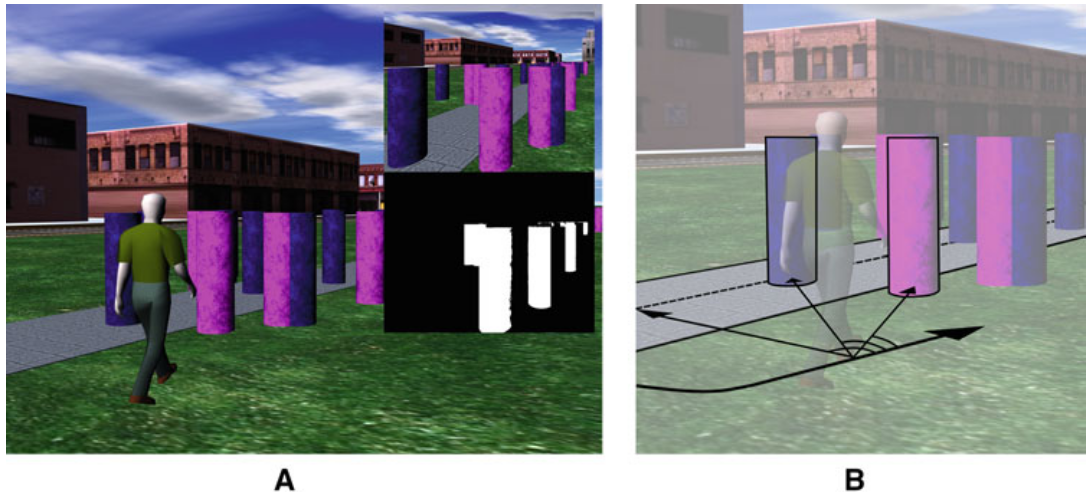
\includegraphics[width=0.6\textwidth]{avatar.png}
\caption{The task of collecting targets, avoiding obstacles and following the
path.}
\label{fig:avatar}
\end{figure}

Consider the task illustrated in Figure~\ref{fig:avatar} A). The avatar is asked to
do three sub-tasks simultaneously --- 1) following the path, indicated by the gray
line on the ground, 2) getting targets, the blue cylinders, and 3) avoiding
obstacles, the pink cylinders. This is an experiment design used in the
literature to evaluate modular reinforcement learning \cite{rothkopf2013modular}.

From the reinforcement learning perspective, this task can be decomposed to be
three sub-tasks as described above.  In Figure~\ref{fig:avatar} B), if the agent
knows the distance and angle to an object, he is expected to know the optimal
action to avoid or pursue it.

A human has not done this kind of task before can achieve a good performance
easily, shown in the experiments described later.

\section{Modular Reinforcement Learning}

Value functions is decomposed \cite{koller1999computing}.

 If a human knows the policies
of the sub-tasks, or sub-MDPs, he can accomplish a complicated behavior by
combining the sub-MDPs. That is,
$$Q(s, a) = \sum_i w_i Q_i (s, a)$$
where $Q_i$ is the Q value of the i-th sub-MDP, $w_i$ is the weight of the i-th
sub-MDP. $w_i \geq 0, \sum_i w_i = 1$.

Different weights can yield different performance. Let $w_1, w_2, w_3$ be
weights for the task of target collection, obstacle avoidance, and path
following, respectively. Let $w$ be the vector of $(w_i)_1^n$. An agent with $w
= (1, 0, 0)$ only collect targets, and one with $w = (0, 0.5, 0.5)$ may avoid
the obstacles and follow the path.

To obtain the weights given the samples, we need to use the Inverse Modular
Reinforcement Learning technique \cite{rothkopf2013modular}.

\section{Experiments}

We conducted experiments to ask volunteers to accomplish different tasks and
recorded their trajectories. There are four kind of tasks. Task 1, following the
path only, and ignoring other objects. Task 2, following the path, while avoid
the obstacles. Task 3, following the path, while attain targets when possible.
Task 4, following the path, collecting the targets and avoiding obstacles
simutanously.
The human data are collected by the Center for Perceptual Systems in University
of Texas at Austin.

\begin{figure}[h!]
\centering
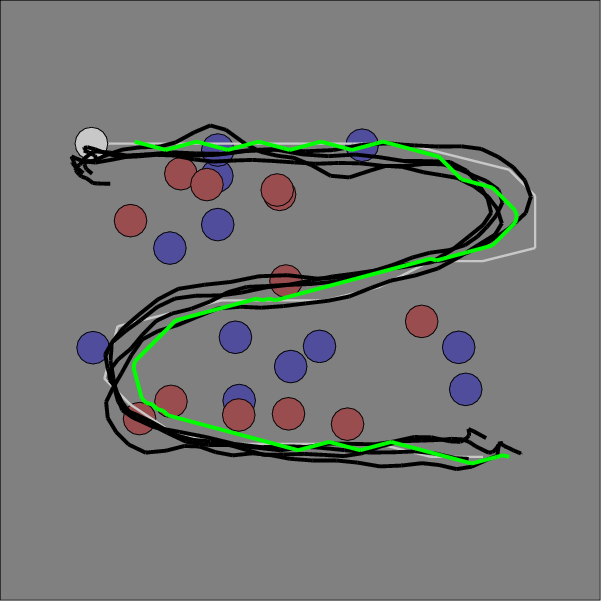
\includegraphics[width=0.24\textwidth]{task_1.png}
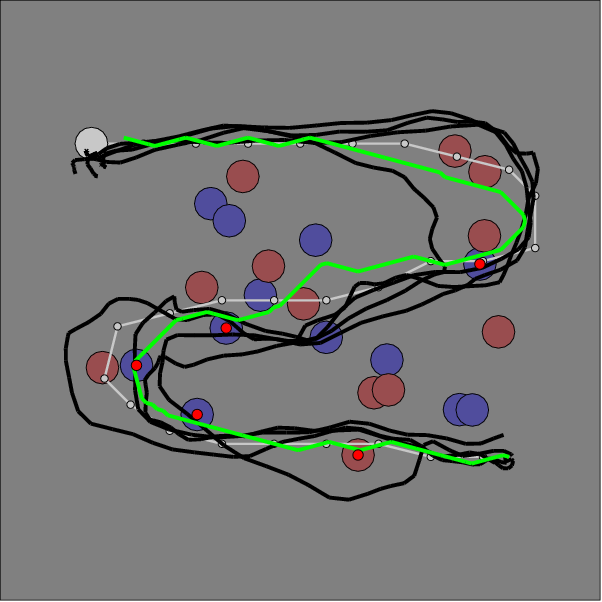
\includegraphics[width=0.24\textwidth]{task_2.png}
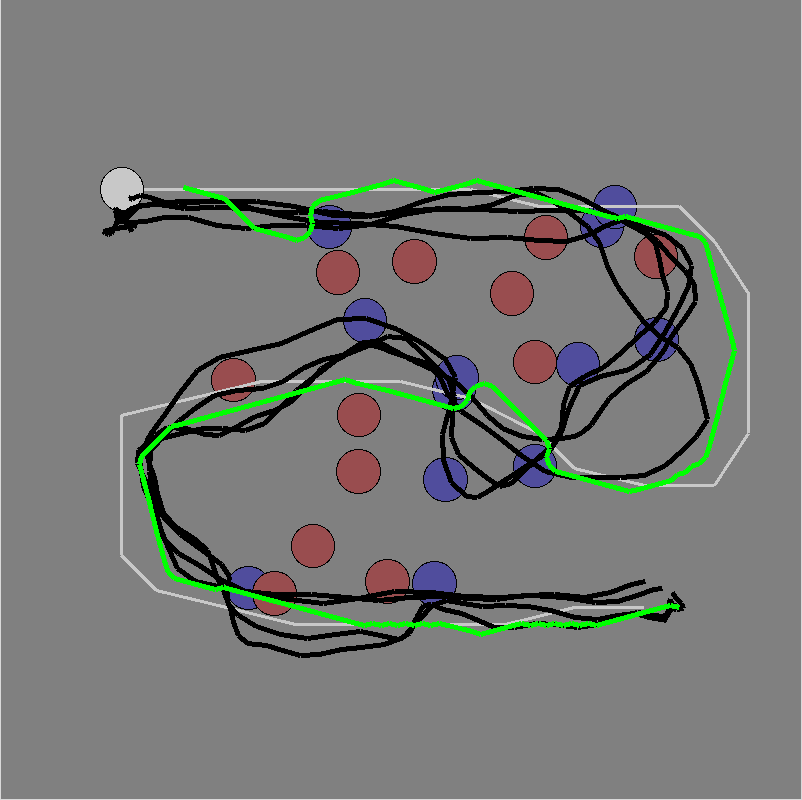
\includegraphics[width=0.24\textwidth]{task_3.png}
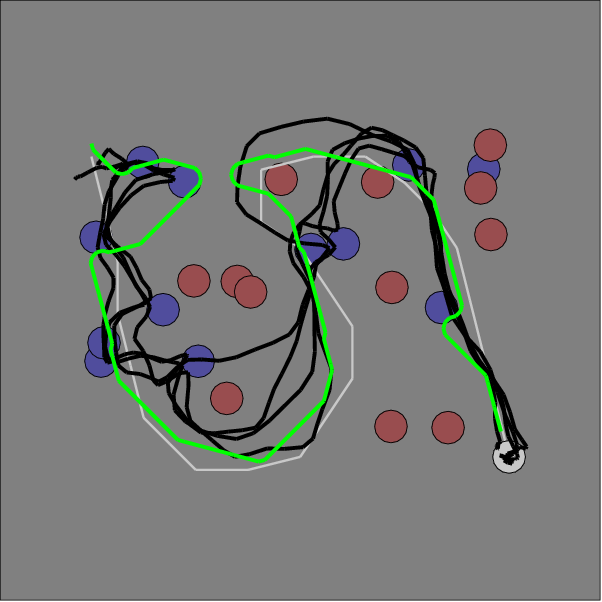
\includegraphics[width=0.24\textwidth]{task_4.png}
\caption{}
\label{fig:exp}
\end{figure}

From a different perspective, can we find a weight vector to best interpret
human's behavior. In Figure~\ref{fig:exp}, same as Figure~\ref{fig:avatar}, the
red circles are obstacles. The blue circles are targets. The gray line is the
path. The black lines are trajectories of human.
%TODO

We make some constraints on our learning agent to make it walk like a human.
We can find in the human trajectories that humans walk smoothly. They don't turn
sharply.  Our agent is allowed to do three actions --- going straight ahead,
turning left with a small step, and turning right with a small step.

To make our weights represent the significance of the modules, we
normalize the sub-MDPs with the unit (positive or negative) rewards. The reward
is 1 for collecting a target, -1 for running into an obstacle. We define the
value function directly for the path module to have a path following performance.

The agent only considers the closest target and the closest obstacle.

We assume that our learning agent only knows the three sub-MDPs and the human
data. It looks at the human behavior, and finds the weights that can interpret
such behavior. 
Using such weights, the trajectories of our agents are drawn in the green lines.
We can tell that in the left figure, the agent puts a large weight on
path-following.  In the right figure, it puts weights on all sub-MDPs.

\begin{figure}[h!]
\centering
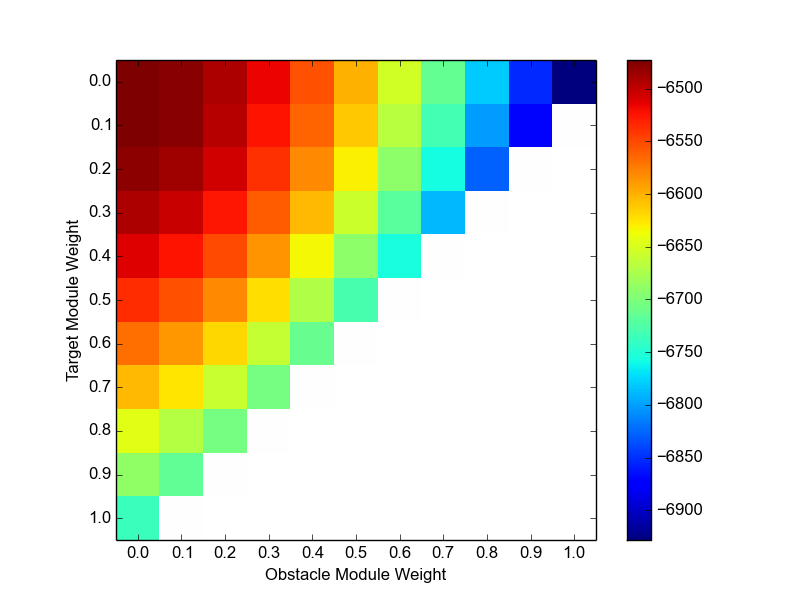
\includegraphics[width=0.4\textwidth]{objValuesTask1.png}
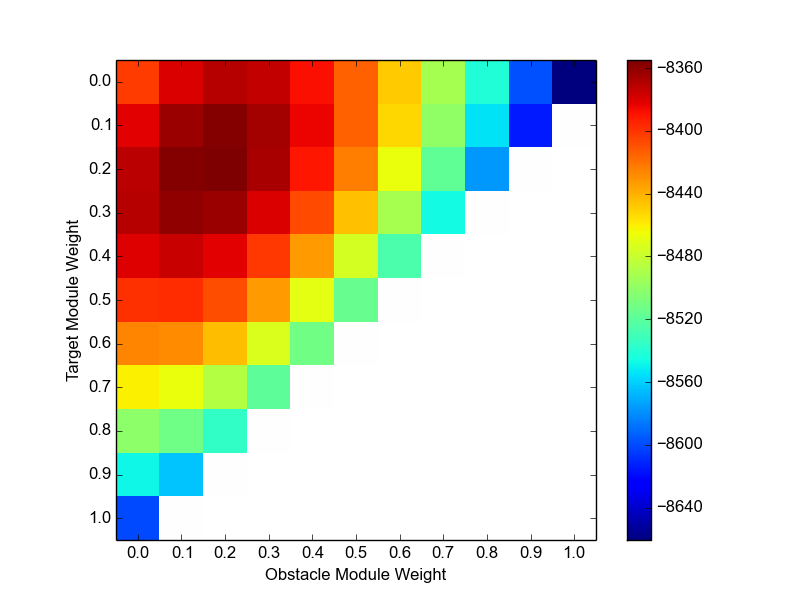
\includegraphics[width=0.4\textwidth]{objValuesTask2.png}
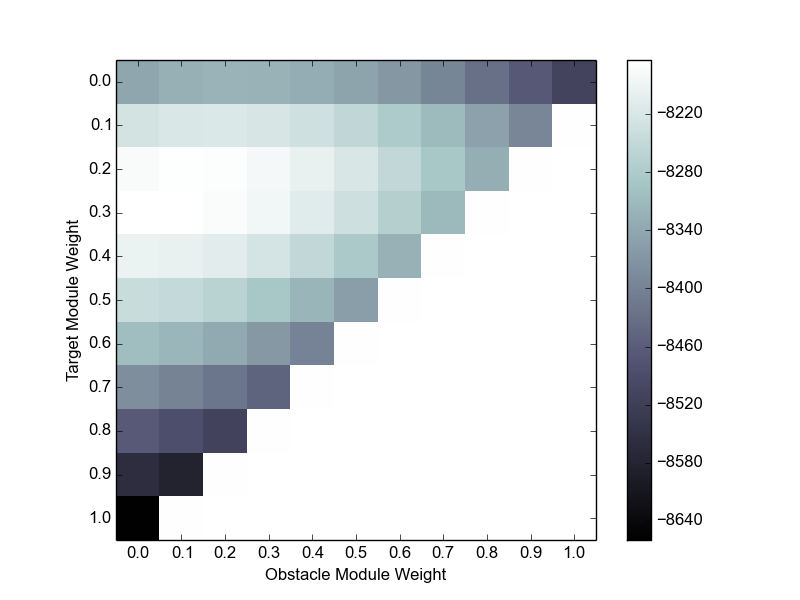
\includegraphics[width=0.4\textwidth]{objValuesTask3.png}
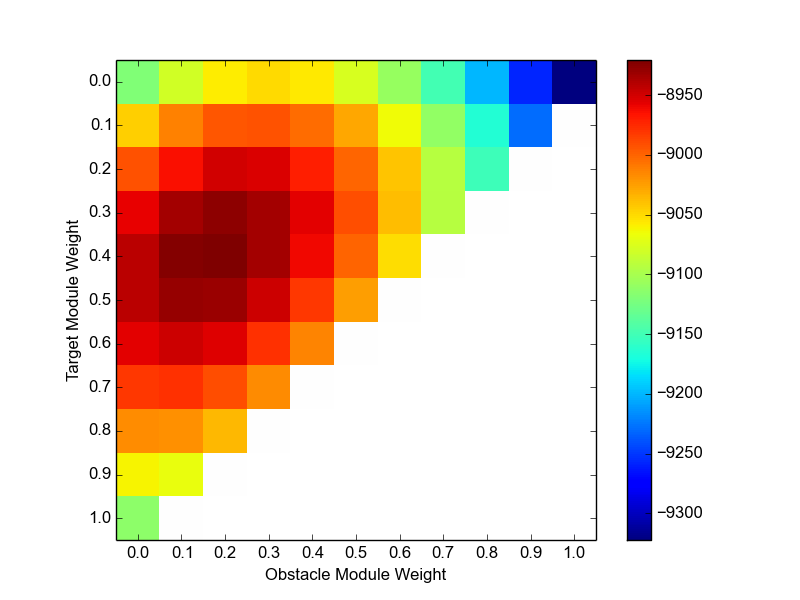
\includegraphics[width=0.4\textwidth]{objValuesTask4.png}
\caption{Heatmaps of the objective values of different weights for the four
tasks, respectively. The red zones indicate higher values. The upper two are
Task 1 and 2. The lower two are Task 3 and 4.}
\label{fig:heatmap}
\end{figure}

\begin{table}[h]
\centering
\begin{tabular}{| l| l| l |}
\hline
Average by Task & Num Targs Hit & Num Obst Hit\\
\hline
1 & 2.34 &  2.13\\
\hline
2 & 3.03 &  \bf{0.13}\\
\hline
3 & \bf{10.19} & 2.28\\
\hline
4 & \bf{9.88} &  \bf{0.03}\\
\hline
\end{tabular}
\caption{Number of targets hit and number of obstacles hit of human.}
\end{table}

\begin{table}[h]
\centering
\begin{tabular}{| l| l| l |}
\hline
Average by Task & Num Targs Hit & Num Obst Hit\\
\hline
1 & 1.25 & 1.62\\
\hline
2 & 3.62 & \bf{2.37}\\
\hline
3 & \bf{5.14} & 3.14\\
\hline
4 & \bf{5.00} & \bf{2.00}\\
\hline
\end{tabular}
\caption{Number of targets hit and number of obstacles hit of the learning agent.}
\end{table}

In Figure~\ref{fig:heatmap}, we show the object values for different weights.

\section{Conclusion and Future Work}

Weighted sum of Q function is one way to combine multiple sub-MDPs. We also
propose other ways including, for example, scheduling between different modules,
with only one active at one time. However, we adopt the weighted sum approach
because this is more reasonble for human behavior. When a human tries to collect
targets while avoiding obstacles, these two modules are expected to be both
active. A scheduling approach may yield frequent oscination between these two
modules.

We also assumes independency between modules. Correlation between modules
doesn't impair our analysis in this paper. In Figure~\ref{fig:heatmap}, we can
find that the target module and obstacle module tends to be negatively
correlated.

\bibliographystyle{plain}
\bibliography{paper}

\end{document}
